%%%%%%%%%%%%%%%%%%%%%%%%%%%%%%%%%%%%%%%%%%%%%%%%%%%%%%%%%%%%%%%%%%%%%%%
%%   TEMPLATE FOR GRADUATE OFFICE                                    %%
%%   UNIVERSIDAD DE PUERTO RICO		       			                 %%
%% 	          MAYAGUEZ                                               %%
%%%%%%%%%%%%%%%%%%%%%%%%%%%%%%%%%%%%%%%%%%%%%%%%%%%%%%%%%%%%%%%%%%%%%%%

% This file defines important information for the thesis,
% Graduate Commitee and the Author.
%%%%%%%%%%%%%%%%%%%%%%%%%%%%%%%%%%%%%%%%%%%%%%%%%%%%%%%%%%%%%%%%%%%%%%%%
%% THIS FILE SPECIFIES ALL INFORMATION OF THE AUTHOR AND THE THESIS
%%
%% This program may be distributed and/or modified under the
%% conditions of the LaTeX Project Public License, either version 1.2
%% of this license or (at your option) any later version.
%% The latest version of this license is in
%%   http://www.latex-project.org/lppl.txt
%% and version 1.2 or later is part of all distributions of LaTeX
%% version 1999/12/01 or later.
%%
%%%%%%%%%%%%%%%%%%%%%%%%%%%%%%%%%%%%%%%%%%%%%%%%%%%%%%%%%%%%%%%%%%%%%%%%

%% This is the definition of the work thesis and the packages that the Thesis 
%% will gonna use

\documentclass[12pt,Bold,Justify,letterpaper]{uprmclass}
\usepackage[dvips,final]{graphicx}
%\usepackage[spanish,activeacute]{babel}
\usepackage{amssymb,amsmath,amsthm,mathrsfs,keyval,color,psfrag,multirow,lscape}		%,overcite}
%\usepackage{calrsfs} 			% beatiful curly letters
\usepackage[bookmarks=true,bookmarksopen=true,breaklinks=true,letterpaper=true,pdftitle={DCFFT},plainpages=false,pdfauthor={StudentRUM},colorlinks=true,hypertexnames=false,citecolor=blue,linkcolor=blue,filecolor=blue]{hyperref}
%\usepackage[pdfpagemode={UseOutlines},bookmarks=true,bookmarksopen=true,bookmarksopenlevel=0,bookmarksnumbered=true,hypertexnames=false,colorlinks=true,linkcolor={blue},citecolor={blue},urlcolor={cyan},pdfstartview={FitV},unicode,breaklinks=true,linktocpage]{hyperref}
\usepackage[numbers,sort&compress]{natbib}
\usepackage{hypernat}
\usepackage{graphics}
\usepackage{rotating}   	% Package for rotate tables
%\usepackage{subfigure}  	% If you want subfigures


%%%%%%%%%%%%%%%%%%%%%%%%%%%%%%%%%%%%%%%%%%%%%%%
%% DEFINE STUDENT AND THESIS SPECIFIC INFO   %%
%%%%%%%%%%%%%%%%%%%%%%%%%%%%%%%%%%%%%%%%%%%%%%%
\SetFullName{William J. Navas-Auger}
\SetThesisType{Dissertation}
\SetThesisTypes{Disertaci\'on}
\SetDegreeType{Doctor of Philosophy}		
\SetDegreeTypes{Doctor en Filosof\'ia}
\SetSpecialty{Computing and Information Science and Engineering}
\SetGradMonth{May}
\SetGradMes{Mayo}
\SetGradYear{2021}
\SetDepartment{Computer Science and Engineering}
\SetDepartmento{Ciencia de Computadoras e Ingenier\'ia}
\SetChair{Vidya Manian}
\SetTitle{SPATIAL ADAPTIVE TENSOR FACTORIZATION FOR HYPERSPECTRAL IMAGE UNMIXING}
\SetTitlesp{Factorizacion Espacial-Adaptiva de Tensores para la separacion de Im\'agenes Hiperespectrales}

%% Signature page members
% First Member Graduate Commitee
\SetNamea{Emmanuel Arzuaga}		
\SetDegreea{Ph.D}
% Second Member Graduate Commitee
\SetNameb{Heidi Sierra}
\SetDegreeb{Ph.D}
% President Graduate Commitee (Normally Chairman)
\SetNamec{Vidya Manian}			
\SetDegreec{Ph.D}
% Graduate Studies Representative
\SetNamed{Graduate Studies Representative}
\SetDegreed{Ph.D.}
% Chairperson of the Department
\SetNameChairDep{Emanuel Arzuaga}
\SetDegreeChairDep{Ph.D}

% This file contents all the commands of style defined for the thesis such as theorems,
% definitions, etc... (if you have no idea what is it. Don't modify anything)
% def.tex is a file used to define special enviroments such as a proof of a theorem.
% defs.tex
%==========================================================================

\theoremstyle{plain}
\newtheorem{definition}[subsection]{Definition} % This defines the Definition enviroment
												% Ver capitulo 5.
\newtheorem*{example}{Example}					% This is example
												% Ver capitulo 5.

\newtheorem{theorem}{Theorem}	% This is the theorem formulation heading
								% Ver capitulo 5.

\newtheorem*{proofa}{Proof}

\hypersetup{urlcolor=blue}		% Especifica el azul para los hypervinculos. (pags web)

\newcommand{\fn}[1]{\texttt{#1}} % Estas dos lineas son utiles para el capitulo 4.
\newcommand{\cn}[1]{\texttt{\char92 #1}}     	 

\begin{document}

% Set format for preliminary pages and roman numbers pagination.
\frontmatter							

% Creates the signature page, abstract(english, spanish),
% copyright, dedication, and acknowledgements pages.
%%%%%%%%%%%%%%%%%%%%%%%%%%%%%%%%%%%%%%%%%%
%%  Make the Introduction of the thesis %%
%%%%%%%%%%%%%%%%%%%%%%%%%%%%%%%%%%%%%%%%%%

%Signature page
\maketitle

% Abstract in English
\abstracte{% Abstract_eng.tex
% Abstract in English
%==========================================================================

\bigskip  % Don't delete this it left a little space between header and the abstract.

This is the Abstract in English. You must write it in the file: 

\vspace{0.5in}

\begin{center}
	\begin{verbatim}Abstracteng.tex .
	\end{verbatim}
\end{center}
}

% Abstract in Spanish
\abstracts{% Abstract_esp.tex
% Abstract in Spanish
%==========================================================================

\bigskip   % No borre esto. Esto deja un espacio entre el encabezado y el cuerpo del resumen

Este es el resumen en Espa\~nol. Usted debe escribirlo en el archivo: 

\vspace{.5in}

\begin{center}
	\begin{verbatim}Abstractesp.tex
	\end{verbatim}
\end{center}

}

% Copyright page
\makecopyright 

% Dedication page
\dedication{%%%%%%%%%%%%%%%%%%%%%%%%%%%%%
%         Dedication        %
%%%%%%%%%%%%%%%%%%%%%%%%%%%%%

You can put the dedication HERE.
\par

Use the file: 
\begin{verbatim} dedication.tex
\end{verbatim}
}

% Acknowledge page
\acknowledge{% Acknowledgements.tex

To Alberto Santana from Chemistry Department who gave me the first version of this template.\par

To Professor Manuel Jimenez (INEL) who push me in the world of \LaTeX.

My chairman Prof Domingo Rodriguez who encourage my work in \LaTeX.

Use the file: 

\begin{verbatim}
Abstracteng.tex .
\end{verbatim}
}


% Generate indices
\tableofcontents					
\listoftables 						
\listoffigures

% Glosary of abbrev. and symbols 						
%%%%%%%%%%%%%%%%%%%%%%%%%%%%%%%%%
%%% List of Abbreviations %%%%%%%
%%%%%%%%%%%%%%%%%%%%%%%%%%%%%%%%%
\chapter*{LIST OF ABBREVIATIONS}
\addcontentsline{toc}{extrachapter}{LIST OF ABBREVIATIONS}%

\begin{symbollist*}

\item[FFT]  Fast Fourier Transform.
\item[DCFT] Discrete Chirp Fourier Transform.


\end{symbollist*}
%%%%%%%%%%%%%%%%%%%%%%%%%%%%%%%%%
%%% List of Symbols %%%%%%%
%%%%%%%%%%%%%%%%%%%%%%%%%%%%%%%%%
\chapter*{LIST OF SYMBOLS}
\addcontentsline{toc}{extrachapter}{LIST OF SYMBOLS}%

\begin{symbollist}[0.7in]

\item[t]      Time (seconds)
\item[$\tau$] Time between events.
\item[$\mu$g] Micrograms.

\end{symbollist}	

% Begin main body of the thesis. 
% Change line numbering from i,ii, to 1,2 
\mainmatter							 
% Introduction.tex
%==========================================================================
\chapter{INTRODUCTION}  % En Mayusculas (In Caps)

The first chapter begins here.

\section{First section of Chapter 1}

En esta secci\'on haremos un ejemplo para ilustrar los temas que tiene esta plantilla.

\begin{example}
Esto es una demostracion de un ejemplo.
\end{example}

\section{Example of paper citation}

As mention the paper \cite{Cohen85} 

% chapter2.tex
%==========================================================================
\chapter{TITLE OF CHAPTER 2}  % En Mayusculas (In Caps)

Here goes the text of Chapter 2.

\section{Example of a figure}

\begin{figure}[ht]
\begin{center}
	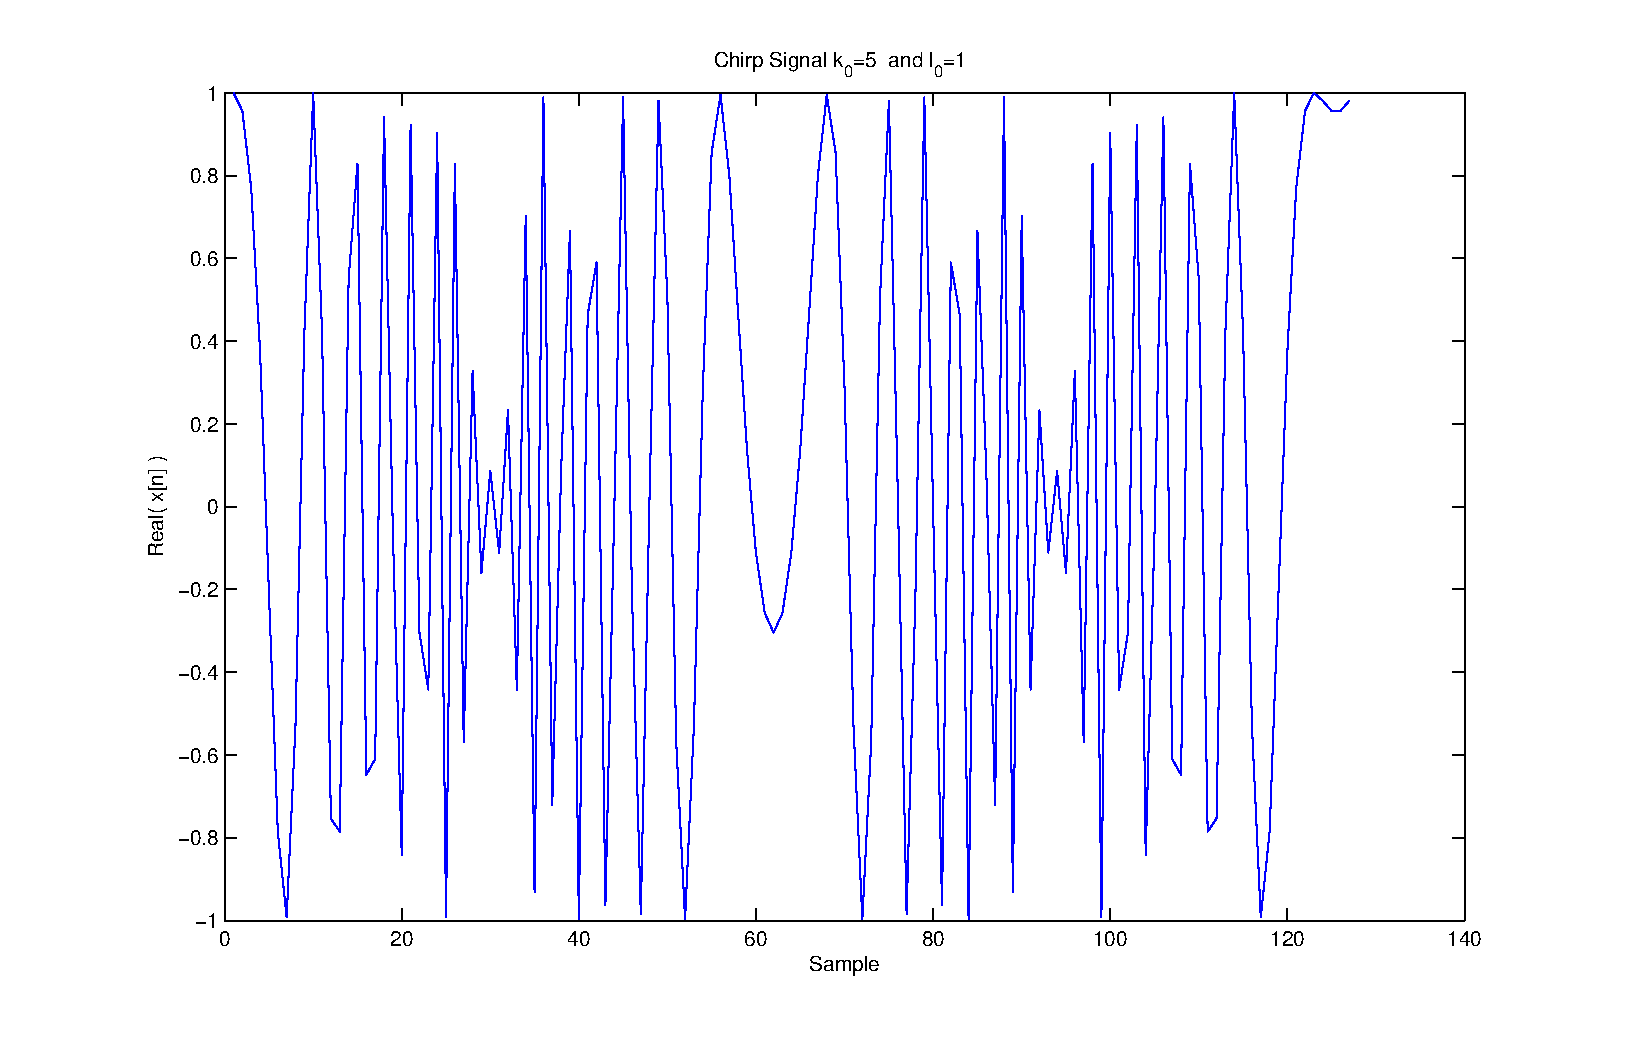
\includegraphics[width=5in]{figs/Chirpsignal}
	\caption{Chirp Signal}
	\label{fig:Chirpsig}
\end{center}
\end{figure}
% chapter3.tex
%==========================================================================
\chapter{TITLE OF CHAPTER 3} % En Mayusculas (In Caps)

\section{Just some about formulas}

Use of \fn{equation*}:

\begin{equation*}
a=b
\end{equation*}

Use of \fn{equation}:

\begin{equation}
a=b
\end{equation}

Use of \fn{split} and \fn{equation}:

\begin{equation}\label{xx}
\begin{split}
a& =b+c-d\\
& \quad +e-f\\
& =g+h\\
& =i
\end{split}
\end{equation}

Use of \fn{multline}:

\begin{multline}
a+b+c+d+e+f+b+c+d+e+f+b+c+d+e+f\\
+b+c+d+e+f+b+c+d+e+f+i+j+k+l+m+n
\end{multline}

Use of \fn{gather}:

\begin{gather}
a_1=b_1+c_1\\
a_2=b_2+c_2-d_2+e_2 \label{eq:D}
\end{gather}

Use of \fn{align}:

\begin{align}
a_1& =b_1+c_1\\
a_2& =b_2+c_2-d_2+e_2
\end{align}

Other uses for \fn{align}:

\begin{align}
a_{11}& =b_{11}&
a_{12}& =b_{12}\\
a_{21}& =b_{21}&
a_{22}& =b_{22}+c_{22}
\end{align}

Use of \fn{flalign*}:

\begin{flalign*}
a_{11}& =b_{11}&
a_{12}& =b_{12}\\
a_{21}& =b_{21}&
a_{22}& =b_{22}+c_{22}
\end{flalign*}

Use of \cn{equation} and \cn{split}:

\begin{equation}\label{e:barwq}\begin{split}
H_c&=\frac{1}{2n} \sum^n_{l=0}(-1)^{l}(n-{l})^{p-2}
\sum_{l _1+\dots+ l _p=l}\prod^p_{i=1} \binom{n_i}{l _i}\\
&\quad\cdot[(n-l )-(n_i-l _i)]^{n_i-l _i}\cdot \Bigl[(n-l
)^2-\sum^p_{j=1}(n_i-l _i)^2\Bigr].
\end{split}\end{equation}

Use of \cn{align} to align textual annotations:

\begin{align}
x& = y_1-y_2+y_3-y_5+y_8-\dots
&& \text{by \eqref{eq:C}}\\
& = y \circ y^* && \text{by \eqref{eq:D}}\\
& = y(0) y && \text {by Axiom 1.}
\end{align}

Use of \cn{aligned} to control placement of inner alignments:

\begin{equation*}
\begin{aligned}
\alpha&=\alpha\alpha\\
\beta&=\beta\beta\beta\beta\beta\\
\gamma&=\gamma
\end{aligned}
\qquad\text{versus}\qquad
\begin{aligned}[t]
\delta&=\delta\delta\\
\eta&=\eta\eta\eta\eta\eta\eta\\
\varphi&=\varphi
\end{aligned}
\end{equation*}

``Cases" constructions:

\begin{equation}\label{eq:C}
P_{r-j}=
\begin{cases}
0& \text{if $r-j$ is odd},\\
r!\,(-1)^{(r-j)/2}& \text{if $r-j$ is even}.
\end{cases}
\end{equation}

Use of \cn{smash} and \cn{vphantom} to control vertical size:

\newcommand\ip[2]{\langle #1 \/ | #2 \/\rangle}
\newcommand\Ip[2]{\left\langle{\arraycolsep=0pt %
\begin{array}{c|c}#1\/\,&\,#2\/\end{array}}%
\right\rangle}
\newcommand\Ipd[2]{\left\langle{\arraycolsep=0pt %
\begin{array}{c|c}\displaystyle#1\/\,&\,\displaystyle#2\/\end{array}}%
\right\rangle}
\newcommand\conj[1]{\overline{#1}}
\begin{align*}
\Ipd{ u\: }{\: \smash{\sum_{i=1}^n F(e_i,v) e_i }\vphantom{\sum}}
&= \sum_{i=1}^n F(e_i,v) \ip{ u }{ e_i } \\
&= \sum_{i=1}^n \ip{ u }{ e_i } F(e_i,v) \\
&= \sum_{i=1}^n \conj{\ip{ e_i }{ u }} F(e_i,v) \\
&= F \biggl( \sum_{i=1}^n \ip{ e_i }{ u } e_i,v\biggr) = F( u, v
),
\end{align*}
% chapter4.tex
%==========================================================================
\chapter{TITLE OF CHAPTER 4}  % En Mayusculas (In Caps)

This is the chapter 4.

\section{How to write tables}

\begin{example}
A little table (see table \ref{products}) :


\begin{table}[ht]
\vspace{.2in}
\caption{Benchmark Computational operations for the DCFT vs DFT}
\begin{center}
	\begin{tabular}{|c|c|c|c|}
	  \hline
	 Samples & DCFT & DFT & Cooley-Tukey FFT \\
	  \hline
	  2 & 8 & 4 & 2 \\
	  4 & 64 & 16 & 8 \\
	  8 & 512 & 64 & 24 \\
	  16 & 4096 & 256 & 64 \\
	  32 & 32768 & 1024 & 160\\
	  64 & 262144 & 4096 & 384\\
	  1024 & 1.0737E9 & 1.04858E6 & 10240 \\
	 \hline
	\end{tabular}\label{products}
	\end{center}
\end{table}

\end{example}
%% chapter5.tex
%==========================================================================
\chapter{CHAPTER 5}


					
%% chapter6.tex
%==========================================================================
\chapter{CHAPTER 6}
              	
% Conclusion.tex
%==========================================================================
\chapter{CONCLUSION AND FUTURE WORKS}


\LaTeX is a powerful tool for writing scientific documents.

This template is forever an unfinished work. Your contributions are important to make a better template. Any improvement could be sent to graduate studies office at the RUM.
    				

% Set formatting for appendix sections
\appendix							 
% Genenerate appendix divider page
\makeappendicespage
% Appendix
%==========================================================================
\chapter{TITLE OF APPENDIX A}
\label{AppA}

Appendix A goes here.

% Appendix
%==========================================================================
\chapter{TITLE OF APPENDIX B}
\label{AppB}


Appendix B goes here.

%%       Make List of References
%%%%%%%%%%%%%%%%%%%%%%%%%%%%%%%%%%%%%%%%%%%%%%%%%%%%%%%%%%%%%%%%
%% Note: I use BibTeX, but have coded in thebibliography environment
%%       to use for this example only.
%%%%%%%%%%%%%%%%%%%%%%%%%%%%%%%%%%%%%%%%%%%%%%%%%%%%%%%%%%%%%%%%

% unstr is the same as plain, but entries appear in the order of citation.
\bibliographystyle{unsrt}
% Use the References.bib file
\bibliography{referencefiles/refs} 		

\backmatter

% Add the Biography pages if you want.
\biography{
% Biography.tex


Here goes the Biography.

Use the file: 
\begin{verbatim}
{Biography.tex}
\end{verbatim}

%%%% CESAR ACEROS %%%% Biography %%%%%

%Cesar A Aceros was born in Dec, 23 of 1970 in Bucaramanga, Santander, Colombia. Cesar is son of Rodolfo Aceros Fajardo and Esperanza Moreno de Aceros. In October of 1995 receive the Electronic Engineer degree from the Pontificia Universidad Javeriana. He works in Conalvidrios S.A. the second in importance bottle glass factory in Colombia and later in August of 1996, he works at the Universidad Pontificia Bolivariana in Bucaramanga as a proffesor. In 2003 he left Colombia and start the M.S. studies at the University of Puerto Rico at Mayag\"uez. 


%%%% ALBERTO SANTANA %%%% Biography %%%%%

%was born on May 2$^{\rm nd}$, 1972, in San Germ\'an, Puerto Rico. Alberto is the son of Radam\'es Santana and N\'elida Vargas. In June 1995 he received his B.S.\ degree in chemistry from the University of Puerto Rico, Mayag\"uez Campus. In August of the same year, he started his graduate education. He worked under the supervision of Dr.\ Samuel P.\ Hern\'andez. Alberto spent more than two years doing research in the area of surface enhanced Raman spectroscopy (SERS). In June of 1998, Alberto received his second academic degree, a M.S.\ in chemistry from the same university.
%
%After doing experimental work, Alberto decided to continue his academic formation, but this time it would be in another area of chemistry. He came to the USA in January of 1998 and joined the Physical Chemistry Division of the Chemistry Department at the University of Florida. After completing his written and oral examinations, Alberto was admitted to the Ph.D.\ program and started his research on the theoretical and computational aspects of quantum molecular dynamics applied to surface chemistry under the supervision of Dr. David A. Micha. 
			
}

%%%%%%%%%%%%%%%%%%%%%%%%%%%%%%%%%%%%%%%%%%%%%%%
%%  Create a General Audience Abstract      %%%
%%%%%%%%%%%%%%%%%%%%%%%%%%%%%%%%%%%%%%%%%%%%%%%

\begin{simpleenv}{}{}{}{}%
\pagestyle{empty}
\begin{flushleft}
\Title\\*[\BaseDiff\baselineskip]
\FullName\\
(787) XXX-XXXX\\
Department of \Department \\
Chair: \Chair\\
Degree: \DegreeType\\
Graduation Date: \GradMonth~\GradYear
\end{flushleft}
\GoDouble
% GeneralAudienceAbstract.tex


This is the general Audience Abstract.

Use the file: \fn{GeneralAudienceAbstract.tex}

%Density matrix theory is applied to the CO/Cu(001)
%adsorbate/substrate system to evaluate the nonlinear photodesorption yield of CO versus pulse fluence through model calculations. The dynamics of molecular photodesorption from a metal surface is described by the nonlinear optical response resulting from the interaction of a femtosecond pulsed laser with a metal surface. Our formalism uses the Liouville-von Neumann equation, with an effective hamiltonian which includes the effects of energy dissipation into the metal. The nonlinear response of the substrate to femtosecond excitation is taken into account by solving modified optical Bloch equations with relaxation terms to account for the effects of energy dissipation. Our previous density matrix treatment has been extended to include several quantum states, and to treat rotational motions of the desorbing molecule. Results for intense lasers including chirping at pulse wavelengths around 620 nm have also been obtained.

\end{simpleenv}

								% This file create the Bibliography, Biography and general abstrac for the thesis.

\end{document}
